\documentclass[12pt, a4paper, oneside, titlepage]{article}
\usepackage{geometry}
\usepackage{fancyhdr}
\usepackage{amsmath, amsthm, amssymb}
\usepackage{graphicx}
\usepackage{hyperref}
\usepackage{array}
\usepackage[english]{babel}
\usepackage[table]{xcolor}
\usepackage{rotating}
\usepackage{multirow}
\usepackage{supertabular}
\usepackage{subfig}
\newcommand{\HRule}{\rule{\linewidth}{0.5mm}}

\pagestyle{fancy}
\fancyhf{}


\fancyhead[RO] {\thepage}
%\fancyhead[LO]{\rightmark}
%\fancyhead[RE]{\leftmark}
%\fancyhead[RE]{\textit{\nouppercase{\leftmark}}}
\fancyhead[LO]{\textit{\nouppercase{\rightmark}}}


\fancypagestyle{plain}{ %
\fancyhf{} % remove everything
\renewcommand{\headrulewidth}{0pt} % remove lines as well
\renewcommand{\footrulewidth}{0pt}}

\begin{document}

\begin{titlepage}
\begin{center}
\thispagestyle{empty}

\textsc{\large Norwegian University of Science and Technology} \\
\textsc{IT3708 - Subsymbolic Methods in AI} \\[3cm]
%\textsc{Group 13} \\[3cm]
\HRule\\[0.5cm]
{\Huge Evolving Spiking-Neuron Parameters}\\[0.5cm]
%\textsc{\large Colonel Blotto}
\HRule\\[3.5cm]

{\large \emph{Author:}}\\
Jonas Eikli\\
Erlend B\o rslid Haugsdal

\vfill

{\large \today}


\end{center}
\end{titlepage}




\addcontentsline{toc}{section}{Contents}
\tableofcontents

\newpage

\section{Introduction}


\section{Description}



\section{Analysis}

The results from the 12 test runs can be seen in Figure \ref{spiketime}, \ref{spikeinterval} and \ref{wave}. Their respective fitness progression can be seen in Figure \ref{spiketimefitness}, \ref{spikeintervalfitness} and \ref{wavefitness}. The fitness graphs shows in what generation there was an improvement to the fitness.

Figure \ref{spiketime} shows all the different test cases made with the Spike Time Distance Metrics. Likewise, Figure \ref{spikeinterval} shows the ones made with Spike Interval Distance Metrics and Figure \ref{wave} shows the ones with Waveform Distance Metrics. 

Table \ref{table} shows the fitness value and the parameters used to make each of the spike trains in the figures.

\begin{table}
	\begin{tabular}{|l|l|l|l|l|l|l|} 
	\hline
	Spike Train & Best fitness & A & B& C& D& K \\ \hline
	Figure \ref{activation1} & 0,74 & 	 0.02609& 0.08030&-48.76832& 1.85161	&0.04096\\
	Figure \ref{activation4} & 0,52	&    0.00100& 0.03636&-78.82697& 8.54838	&0.05645\\
	Figure \ref{activation7} & 0,78&	 0.10721& 0.10411& -49.89247&	 3.10967& 0.0400\\
	Figure \ref{activation10} & 0,40&  	 0.02356& 0.27930& -48.03519& 5.49032&	 0.04677\\ \hline
	Figure \ref{activation2} & 0,40&  	 0.03504& 0.09787& -45.59139&	 6.32258&	 0.04774\\
	Figure \ref{activation5} & 0,67&	 0.00138& 0.03608&	 -75.99217&	 8.61612&	 0.060322\\
	Figure \ref{activation8} & 0,55&	 0.06908& 0.16478& -36.15835&	 6.74838& 0.04000\\
	Figure \ref{activation11} & 0,84&	 0.031346& 0.23735&	 -40.70381&	 4.28064&	 0.040967\\ \hline
	Figure \ref{activation3} & 0,70&	 0.101569& 0.12991&	 -37.38025&	 7.68709&	 0.04000\\
	Figure \ref{activation6} & 0,83&	 0.003139& 0.15259& -57.90811&	 9.95161& 0.07967\\
	Figure \ref{activation9} & 0,86&	 0.003334& 0.01028& -45.24926&	 6.39999& 0.06032\\
	Figure \ref{activation12} &0,80&	 0.003139& 0.12424& -53.90029&	 9.51612& 0.07677\\ \hline
	\end{tabular}
	\caption{The fitness value for, and the parameters used to make, the closest-to-target spike train for each of the 12 test-runs. Note: the values have been rounded off to fit in the table.}
	\label{table}
\end{table}


\begin{figure}
	\centering
	\subfloat[Spike train 1]{\label{activation1}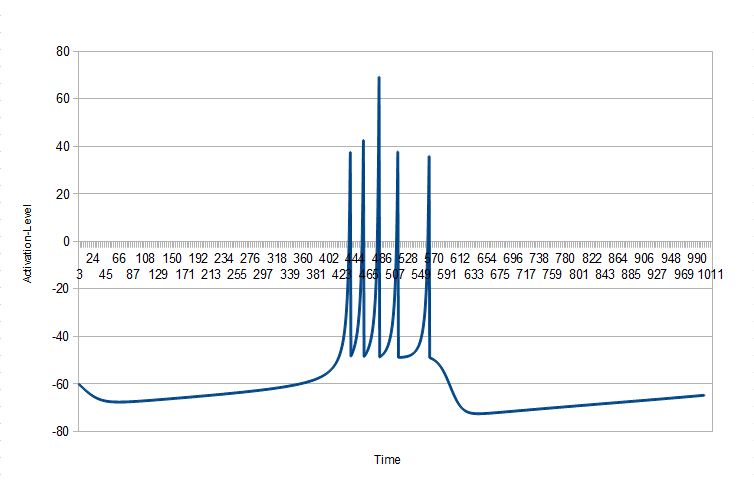
\includegraphics[width=0.5\textwidth]{graphs/activationlevel1}}
	\subfloat[Spike train 2]{\label{activation4}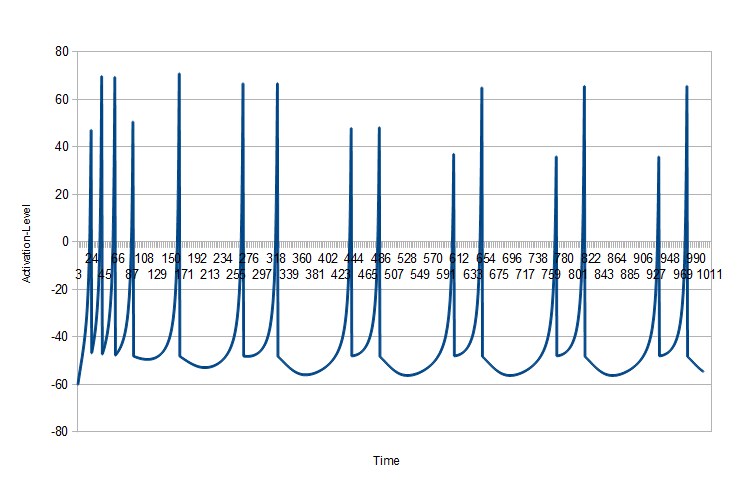
\includegraphics[width=0.5\textwidth]{graphs/activationlevel4}}\\
	\subfloat[Spike train 3]{\label{activation7}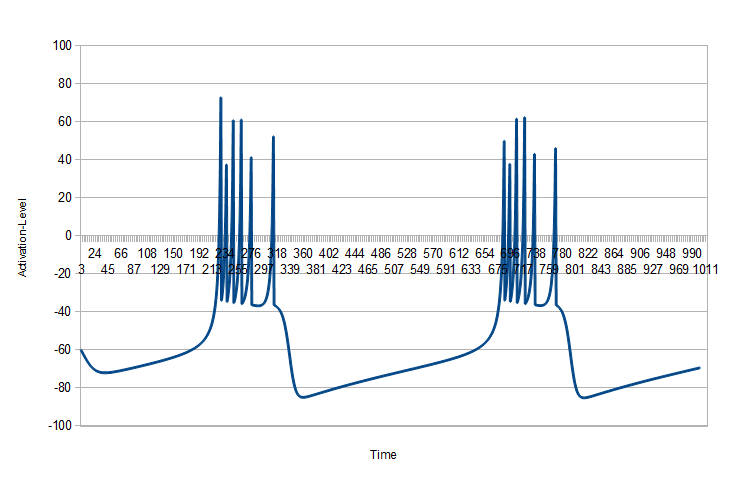
\includegraphics[width=0.5\textwidth]{graphs/activationlevel7}}
	\subfloat[Spike train 4]{\label{activation10}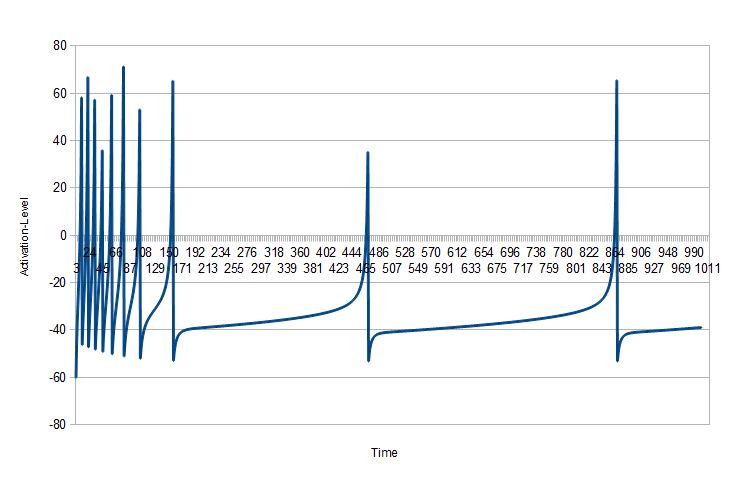
\includegraphics[width=0.5\textwidth]{graphs/activationlevel10}}
	\caption{This is the closest-to-target spike trains developed with Spike Time Distance Metrics.}
	\label{spiketime}
\end{figure}

\begin{figure}
	\centering
	\subfloat[Spike train 1]{\label{fitness1}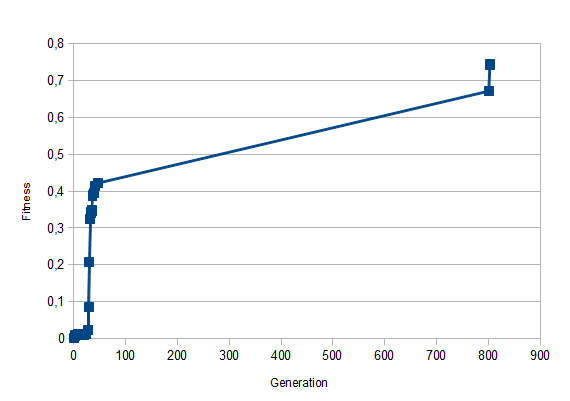
\includegraphics[width=0.5\textwidth]{graphs/fitness1}}
	\subfloat[Spike train 2]{\label{fitness4}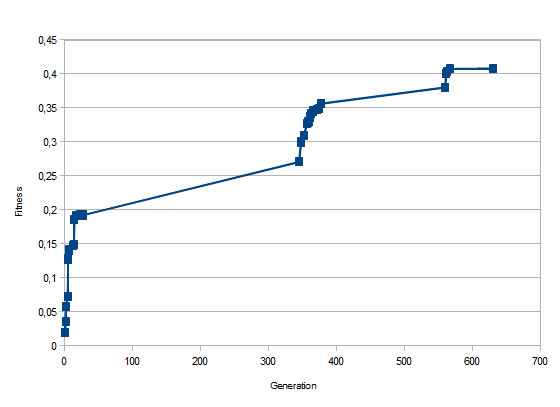
\includegraphics[width=0.5\textwidth]{graphs/fitness4}}\\
	\subfloat[Spike train 3]{\label{fitness7}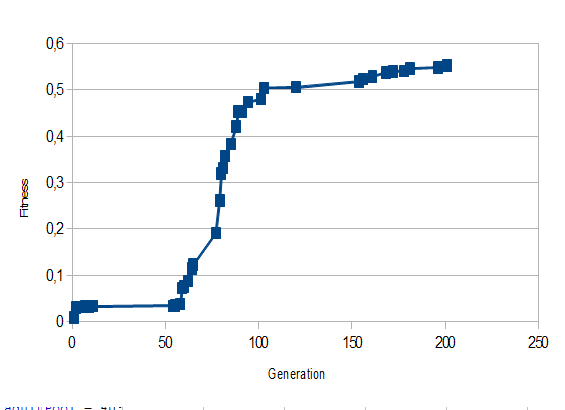
\includegraphics[width=0.5\textwidth]{graphs/fitness7}}
	\subfloat[Spike train 4]{\label{fitness10}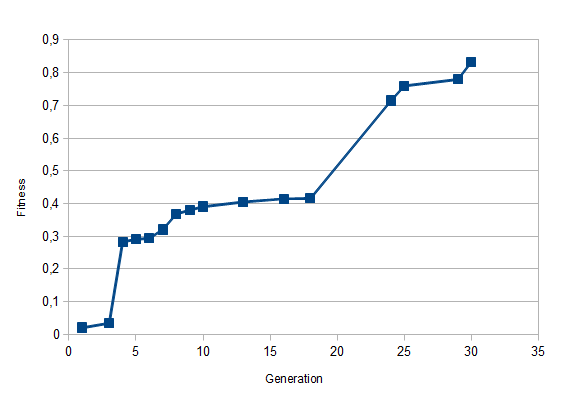
\includegraphics[width=0.5\textwidth]{graphs/fitness10}}
	\caption{This is the fitness graph matching the spike trains developed with Spike Time Distance Metrics.}
	\label{spiketimefitness}
\end{figure}




\begin{figure}
	\centering
	\subfloat[Spike train 1]{\label{activation2}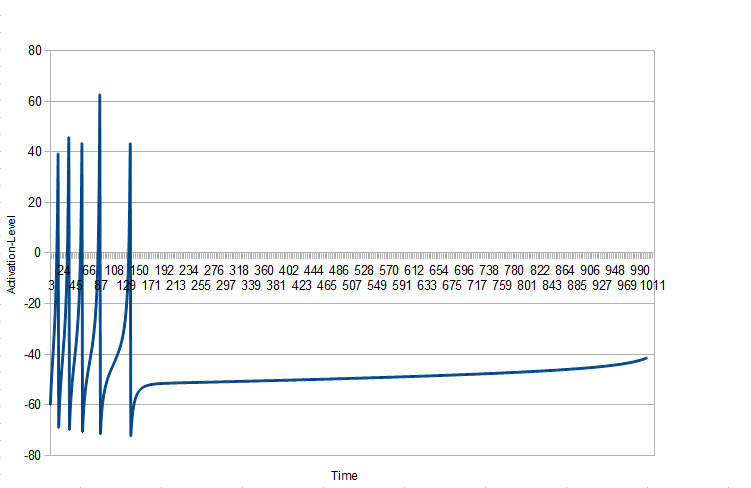
\includegraphics[width=0.5\textwidth]{graphs/activationlevel2}}
	\subfloat[Spike train 2]{\label{activation5}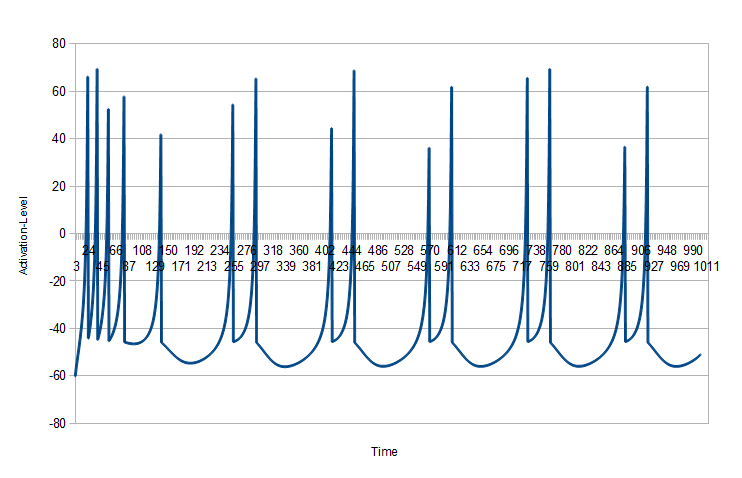
\includegraphics[width=0.5\textwidth]{graphs/activationlevel5}}\\
	\subfloat[Spike train 3]{\label{activation8}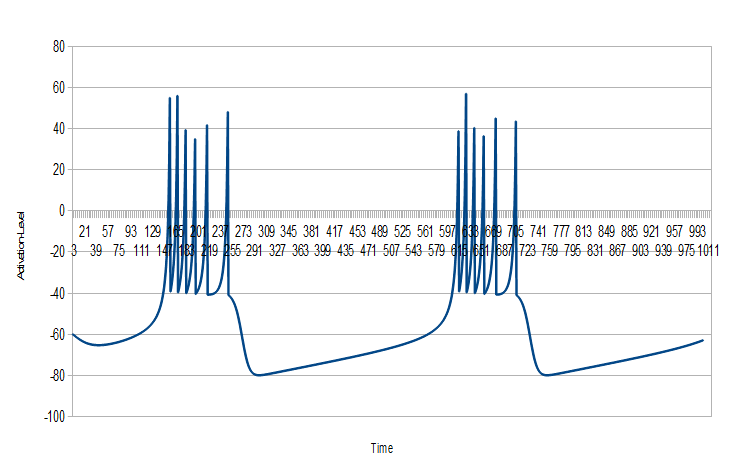
\includegraphics[width=0.5\textwidth]{graphs/activationlevel8}}
	\subfloat[Spike train 4]{\label{activation11}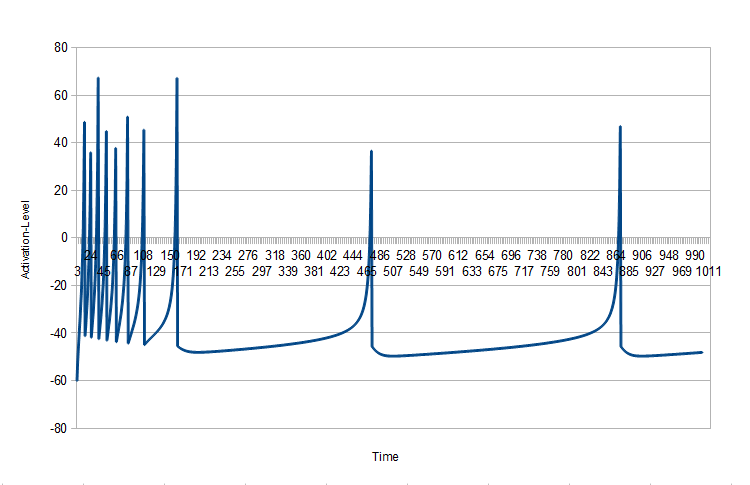
\includegraphics[width=0.5\textwidth]{graphs/activationlevel11}}
	\caption{This is the closest-to-target spike trains developed with Spike Interval Distance Metrics.}
	\label{spikeinterval}
\end{figure}

\begin{figure}
	\centering
	\subfloat[Spike train 1]{\label{fitness2}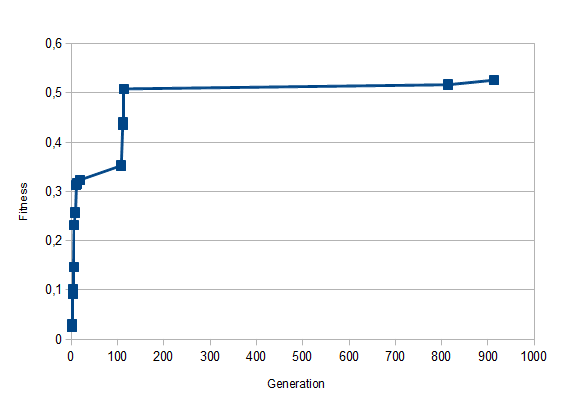
\includegraphics[width=0.5\textwidth]{graphs/fitness2}}
	\subfloat[Spike train 2]{\label{fitness5}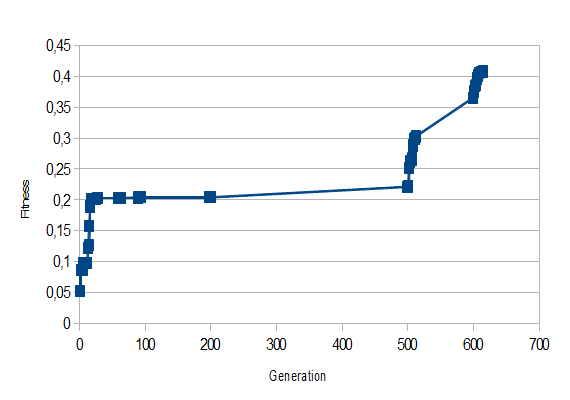
\includegraphics[width=0.5\textwidth]{graphs/fitness5}}\\
	\subfloat[Spike train 3]{\label{fitness8}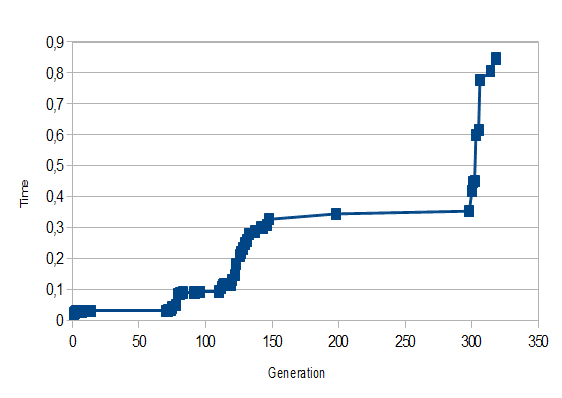
\includegraphics[width=0.5\textwidth]{graphs/fitness8}}
	\subfloat[Spike train 4]{\label{fitness11}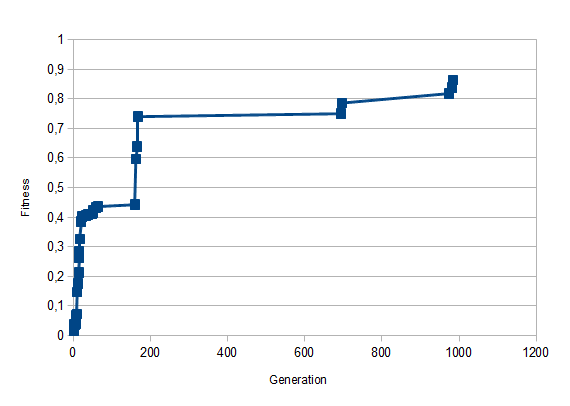
\includegraphics[width=0.5\textwidth]{graphs/fitness11}}
	\caption{This is the fitness graph matching the spike trains developed with Spike Interval Distance Metrics.}
	\label{spikeintervalfitness}
\end{figure}





\begin{figure}
	\centering
	\subfloat[Spike train 1]{\label{activation3}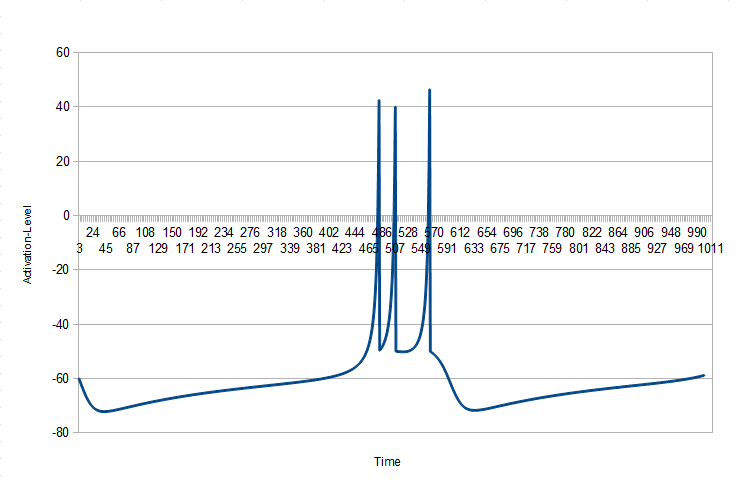
\includegraphics[width=0.5\textwidth]{graphs/activationlevel3}}
	\subfloat[Spike train 2]{\label{activation6}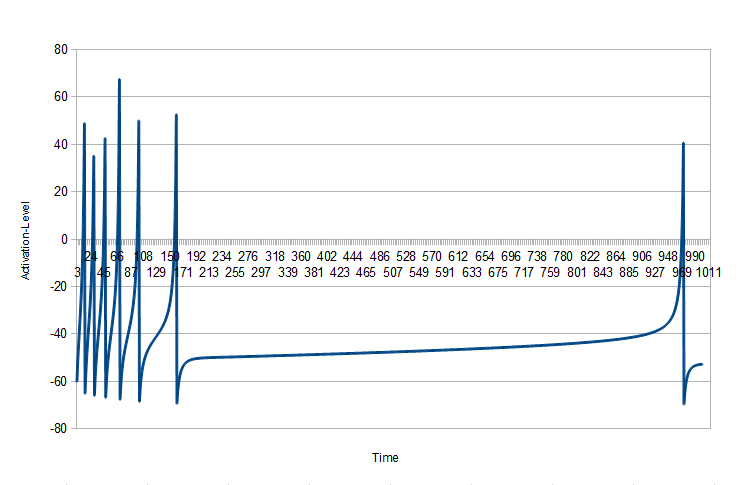
\includegraphics[width=0.5\textwidth]{graphs/activationlevel6}}\\
	\subfloat[Spike train 3]{\label{activation9}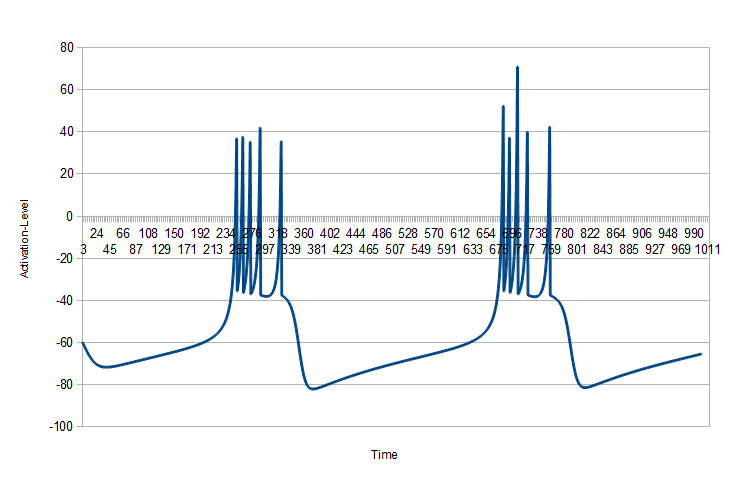
\includegraphics[width=0.5\textwidth]{graphs/activationlevel9}}
	\subfloat[Spike train 4]{\label{activation12}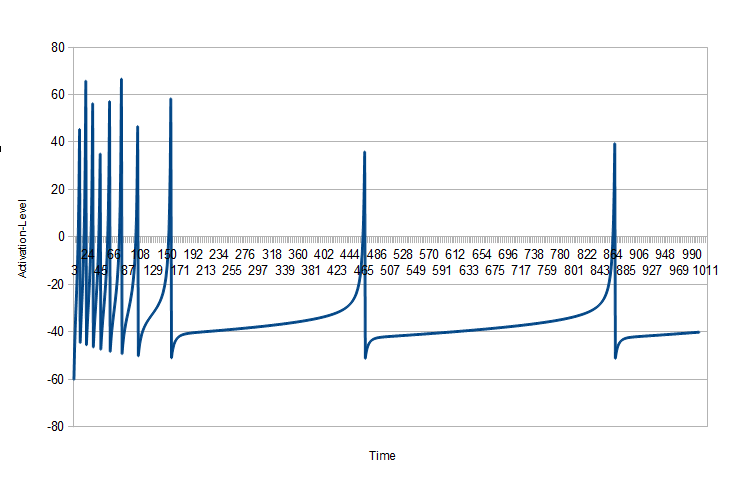
\includegraphics[width=0.5\textwidth]{graphs/activationlevel12}}
	\caption{This is the closest-to-target spike trains developed with Wave Form Distance Metrics.}
	\label{wave}
\end{figure}

\begin{figure}
	\centering
	\subfloat[Spike train 1]{\label{fitness3}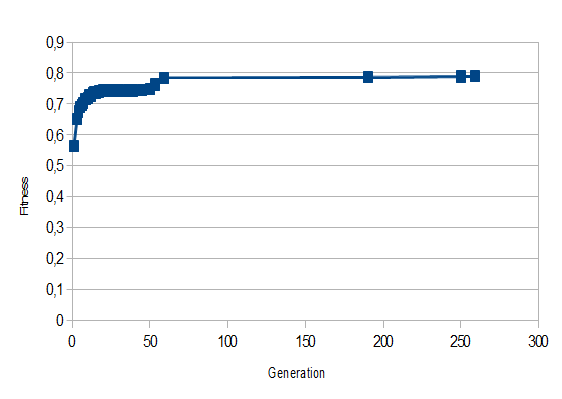
\includegraphics[width=0.5\textwidth]{graphs/fitness3}}
	\subfloat[Spike train 2]{\label{fitness6}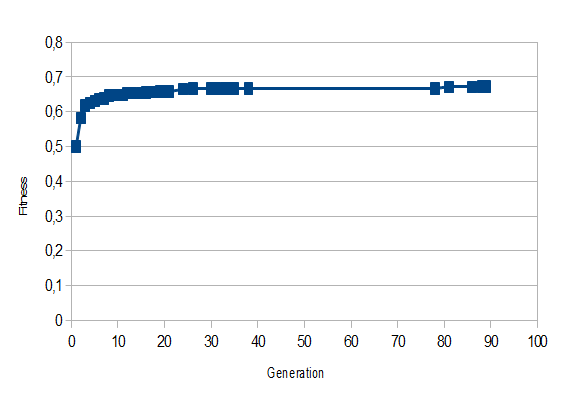
\includegraphics[width=0.5\textwidth]{graphs/fitness6}}\\
	\subfloat[Spike train 3]{\label{fitness9}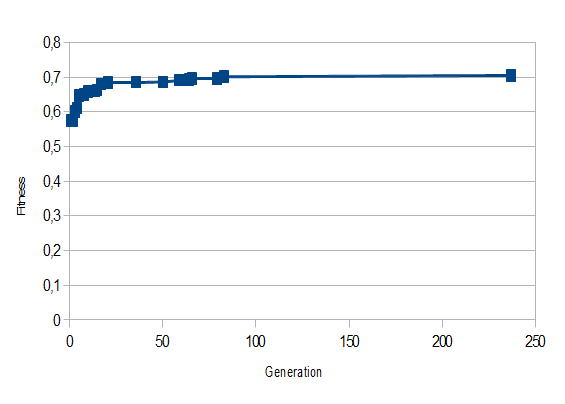
\includegraphics[width=0.5\textwidth]{graphs/fitness9}}
	\subfloat[Spike train 4]{\label{fitness12}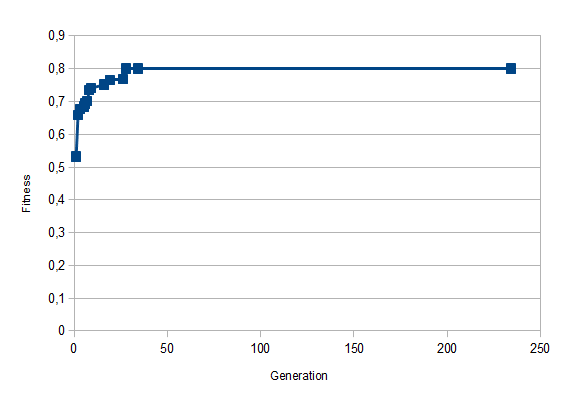
\includegraphics[width=0.5\textwidth]{graphs/fitness12}}
	\caption{This is the fitness graph matching the spike trains developed with Wave Form Distance Metrics.}
	\label{wavefitness}
\end{figure}
\section{Discussion}

\end{document}